\documentclass[a4paper,11pt]{book}
\usepackage{import}
\usepackage{preamb}

\makeindex

\begin{document}

\small
\begin{multicols}{3}

%\maketitle

\thispagestyle{empty}
\scriptsize
\newpage


\begin{subbox}{subbox}{}
\centering
\Large{\textbf{Network Science   \\ Cheatsheet}}
\end{subbox}

\begin{multibox}{2}
\begin{subbox}{subbox}{}
\centering

\includegraphics[width=0.8\textwidth]{pics/logo.png}
\end{subbox}
\begin{subbox}{subbox}{}
\centering
Made by \\
\large{
Remy Cazabet
}
\end{subbox}
\end{multibox}
% \section{Blocks and Community structure}


\begin{subbox}{subbox}{}
\centering
\Large{\textbf{Networks as Matrices}}
\end{subbox}


\begin{textbox}{Matrices in short}
Matrices are mathematical objects that can be thought as \textit{tables} of numbers. The size of a matrix is expressed as $m \times n$, for a matrix with $m$ rows and $n$ columns. \textbf{The order (row/column) is important}.

\textbf{$M_{ij}$} is a notation representing the element on \textbf{row} $i$ and \textbf{column} $j$.

%\centering

%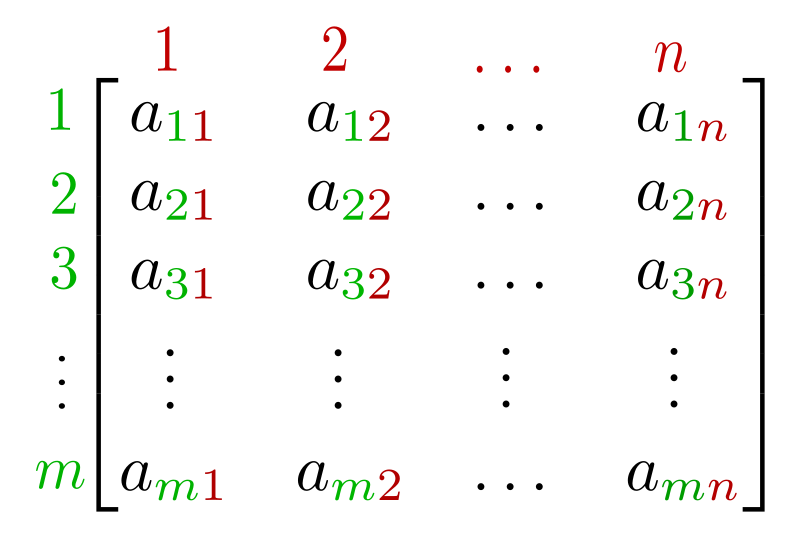
\includegraphics[width=0.5\textwidth]{Matris.png}
%\textbf{Indices in a matrix}
\end{textbox}

\begin{textbox}{$A$ - Adjacency matrix}
The most natural way to represent a graph as a matrix is called the Adjacency matrix $A$. It is defined as a square matrix, such as the number of rows (and the number of columns) is equal to the number of nodes $N$ in the graph. Nodes of the graph are numbered from 1 to $N$, and there is an edge between nodes $i$ and $j$ if the corresponding position of the matrix $A_{ij}$ is not $0$.

\begin{itemize}
    \item A value on the diagonal means that the corresponding node has a \textbf{self-loop}
    \item the graph is \textbf{undirected}, the matrix is \textbf{symmetric}: $A_{ij}=A_{ji}$ for any $i,j$.
    \item In an \textbf{unweighted} network, and edge is represented by the value $1$.
    \item In a \textbf{weighted} network, the value $A_{ij}$ represents the \textbf{weight} of the edge $(i,j)$

\end{itemize}
\end{textbox}


\begin{textbox}{Typical operations on $A$}
Some operations on Adjacency matrices have straightforward interpretations and are frequently used, such as \textbf{Multiplying} $A$ by \textbf{itself} and \textbf{Multiplying} $A$ by a \textbf{column vector}
\end{textbox}


\begin{textbox}{Multiplying $A$ by itself}


\textbf{Multiplying} $A$ by \textbf{itself} allows to know the number of walks of a given length that exist between any pair of nodes: $A^2_{ij}$ corresponds to the number of walks of length 2 from node $i$ to node $j$, $A^3_{ij}$ to the number of walks of length 3, etc.
\end{textbox}

\begin{textbox}{Multiplying $A$ by a column vector}

\textbf{Multiplying} $A$ by a \textbf{column vector} $W$ of length $1\times N$ can be thought as setting the $i$ th value of the vector to the $i$th node, and each node \textit{sending} its value to its neighbors (for undirected graphs). The result is a column vector with $N$ elements, the $i$th element corresponding to the sum of the values of its neighbors in $W$. This is convenient when working with \textbf{random walks} or \textbf{diffusion} phenomenon.
\end{textbox}










\begin{textbox}{Spectral properties of $A$}
\textbf{Spectral Graph Theory} is a whole field in itself, and beyond the scope of this class. A few elements for those with a \textit{linear algebra} background:

\begin{itemize}
    \item The adjacency matrix of an undirected simple graph is symmetric, and therefore has a complete set of real eigenvalues and an orthogonal eigenvector basis.
    \item The set of eigenvalues of a graph is the spectrum of the graph.
    \item The $n$ eigenvalues are denoted as $\lambda_0 \leq \lambda_1 \leq \lambda_2 \leq \dots \lambda_{\max}$
    \item The largest eigenvalue $\lambda_{\max}$ lies between the average and maximum degrees.
    \item In a large, sparse random graph, $\lambda_{\max}\approx \langle k \rangle$
    \item The number of closed walks of length $k$ in $G$ equals $\sum^n_{i=0} \lambda^k_i$
    \item A graph is bipartite if and only if its spectrum is symmetric (i.e., if $\lambda$ is an eigenvalue, then so is $-\lambda$
    \item If $G$ is connected, then the diameter of $G$ is strictly less than its number of distinct eigenvalues
\end{itemize}


\end{textbox}













\begin{textbox}{Graph Laplacian}
The \textbf{Graph Laplacian}, or \textbf{Laplacian Matrix} of a graph is a variant of the Adjacency matrix, often used in \textit{Spectral Graph Theory}.

It is defined as $D-A$, with $D$ the \textit{Degree matrix} of the graph, defined as a $N \times N$ matrix with $D_{ii}=k_i$ and zeros everywhere else.
\end{textbox}































\begin{textbox}{Matrix notation - Example}
\begin{multibox}{2}
\begin{subbox}{white}{\textcolor{black}{Graph}}
\centering
%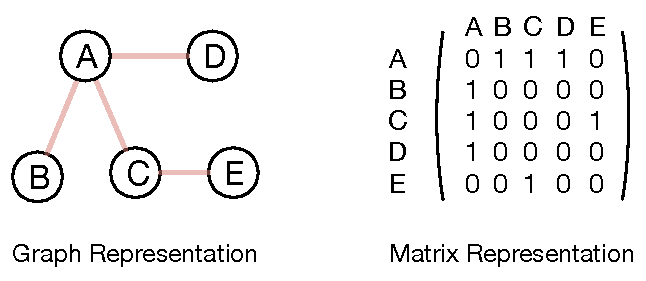
\includegraphics[width=\textwidth]{CheatSheet_pic.pdf}
\adjustbox{width=0.8\textwidth }{
%\scalebox{1}[0.5]{
%\rotatebox[90]{
\begin{tikzpicture}[scale=0.3,rotate=0][every node/.style={inner sep=0,outer sep=0}]
\clip (0,-0.5) rectangle (6,6.5);
\Vertex[x=1.781,y=1.331,size=0.3,opacity=0.8,label=1]{0}
\Vertex[x=3.083,y=3.151,size=0.3,opacity=0.8,label=2]{1}
\Vertex[x=2.831,y=0.200,size=0.3,opacity=0.8,label=6]{5}
\Vertex[x=4.058,y=1.136,size=0.3,opacity=0.8,label=5]{4}
\Vertex[x=4.219,y=5.643,size=0.3,opacity=0.8,label=3]{2}
\Vertex[x=2.386,y=5.800,size=0.3,opacity=0.8,label=4]{3}
\Edge[](0)(1)
\Edge[](0)(5)
\Edge[](0)(4)
\Edge[](1)(2)
\Edge[](1)(3)
\Edge[](1)(4)
\Edge[](1)(5)
\Edge[](5)(4)
\Edge[](4)(4)
\Edge[](2)(3)
\end{tikzpicture}
}%\end{resizebox}
\end{subbox}
\begin{subbox}{white}{\textcolor{black}{$A$ - Adjacency Mat.}}
\centering
\footnotesize
\[\begin{pmatrix}
  0  &  1  &  0  &  0  &  1  &  1 \\
  1  &  0  &  1  &  1  &  1  &  1 \\
  0  &  1  &  0  &  1  &  0  &  0 \\
  0  &  1  &  1  &  0  &  0  &  0 \\
  1  &  1  &  0  &  0  &  1  &  1 \\
  1  &  1  &  0  &  0  &  1  &  0 
\end{pmatrix}
\]
\end{subbox}


\begin{subbox}{white}{\textcolor{black}{$D$ - Degree Matrix}}
\centering
\footnotesize
\[\begin{pmatrix}
  3  &  0  &  0  &  0  &  0  &  0 \\
  0  &  5  &  0  &  0  &  0  &  0 \\
  0  &  0  &  2  &  0  &  0  &  0 \\
  0  &  0  &  0  &  2  &  0  &  0 \\
  0  &  0  &  0  &  0  &  5  &  0 \\
  0  &  0  &  0  &  0  &  0  &  3 
\end{pmatrix}
\]
\end{subbox}
\begin{subbox}{white}{\textcolor{black}{$L$ - Laplacian }}
\centering
\footnotesize
\[
\setlength\arraycolsep{1pt}
\begin{pmatrix}
  3  & -1  &  0  &  0  & -1  & -1 \\
 -1  &  5  & -1  & -1  & -1  & -1 \\
  0  & -1  &  2  & -1  &  0  &  0 \\
  0  & -1  & -1  &  2  &  0  &  0 \\
 -1  & -1  &  0  &  0  &  4  & -1 \\
 -1  & -1  &  0  &  0  & -1  &  3 
\end{pmatrix}
\]
\end{subbox}
\begin{subbox}{white}{\textcolor{black}{ $A^2$}}
\centering
\footnotesize
\[\begin{pmatrix}
  3  &  2  &  1  &  1  &  3  &  2 \\
  2  &  5  &  1  &  1  &  3  &  2 \\
  1  &  1  &  2  &  1  &  1  &  1 \\
  1  &  1  &  1  &  2  &  1  &  1 \\
  3  &  3  &  1  &  1  &  4  &  3 \\
  2  &  2  &  1  &  1  &  3  &  3 
\end{pmatrix}
\]
\end{subbox}
\begin{subbox}{white}{\textcolor{black}{ Random W. mat.}}
\centering
\footnotesize
\setlength\arraycolsep{3pt}
\[\begin{pmatrix}
  0 &  \frac{1}{5} &  0 &  0 &  \frac{1}{4} &  \frac{1}{3}\\[6pt]
  \frac{1}{3} &  0 &  \frac{1}{2} &  \frac{1}{2} &  \frac{1}{4} &  \frac{1}{3}\\[6pt]
  0 &  \frac{1}{5} &  0 &  \frac{1}{2} &  0 &  0\\[6pt]
  0 &  \frac{1}{5} &  \frac{1}{2} &  0 &  0 &  0\\[6pt]
  \frac{1}{3} & \frac{1}{5} &  0 &  0 &  \frac{1}{4} &  \frac{1}{3}\\[6pt]
  \frac{1}{3} &  \frac{1}{5} &  0 &  0 &  \frac{1}{4} &  0
 \end{pmatrix}
\]
\end{subbox}



\end{multibox}
\end{textbox}









\begin{textbox}{Laplace Operator}

Intuitively, the Laplace operator is a generalization of the second derivative, and is defined in discrete situations, for each value, as the sum of differences between the value and its "neighbors". e.g., in time, the 2\textsuperscript{nd} derivative \textit{acceleration} is the difference between current speed and previous speed. In a B\&W picture, it's the difference between the greylevel on current pixel and the greylevel of 4 or 8 closest pixels, and perform \textit{edge detection}. On a graph, with $W$ a column vector representing values on nodes, $LW$ computes for each node the difference to neighbors. 
\end{textbox}




\begin{textbox}{Spectral properties of $L$}
Eigenvalues of the Laplacian have many applications, such as \textit{spectral clustering}, \textit{graph matching}, \textit{embedding}, etc. Assuming $G$ undirected with eigenvalues $\lambda_0 \leq \lambda_1 \leq \lambda_2 \leq \dots \lambda_n$, here are some interesting properties:

\begin{itemize}
    \item The smallest eigenvalue $\lambda_i$ equals 0
    \item The number of 0 eigenvalues gives the number of connected components
\end{itemize}

\end{textbox}


\begin{textbox}{Random Walk matrix}
Another useful matrix of a graph is the \textbf{Random Walk Transition Matrix} $R$. It is the column normalized version of the adjacency matrix. $R_{ij}$ can be understood as the probability for a random walker located on node $i$ to move to $j$.

\end{textbox}


\begin{textbox}{Going Further}
\begin{itemize}
    \item Introduction to spectral graph theory (\cite{nica2016brief})
    \item Survey on Graph Spectral Theory (\cite{spielman2012spectral})

    \item Book on Graph Spectral Theory (\cite{chung1997spectral})
    \item Spectral graph Clustering (\cite{nascimento2011spectral})
    \item Wavelets on graph (\cite{hammond2011wavelets})

\end{itemize}








\end{textbox}





 \AtNextBibliography{\footnotesize}


\printbibliography[heading=subbibliography]


\end{multicols}



\end{document}

